\chapter{Refraction}


The refraction of light is a phenomenon where light changes its direction when it passes from one medium to another. The change in direction is due to a change in the speed of light as it moves from one medium to another. 

This phenomenon is explained by Snell's law, which states:

\begin{equation}
n_1 \cdot \sin(\theta_1) = n_2 \cdot \sin(\theta_2)
\end{equation}

where:
\begin{itemize}
\item $n_1$ and $n_2$ are the indices of refraction for the first and second media, respectively. The index of refraction is the ratio of, $c$ the speed of light in a vacuum to, $v$ the speed of light in the medium, $n=\frac{c}{v}$. It is a dimensionless quantity. $n \ge 1$ for all materials, such that $n_{\text{vacuum}} = 1$ and $n_{\text{air}} \approx 1$. See a list of all mediums here: \url{https://en.wikipedia.org/wiki/List_of_refractive_indices}
\item $\theta_1$ and $\theta_2$ are the angles of incidence and refraction, respectively. These angles are measured from the normal (perpendicular line) to the surface at the point where light hits the boundary.
\end{itemize}

\begin{figure}[htbp]
    \centering
    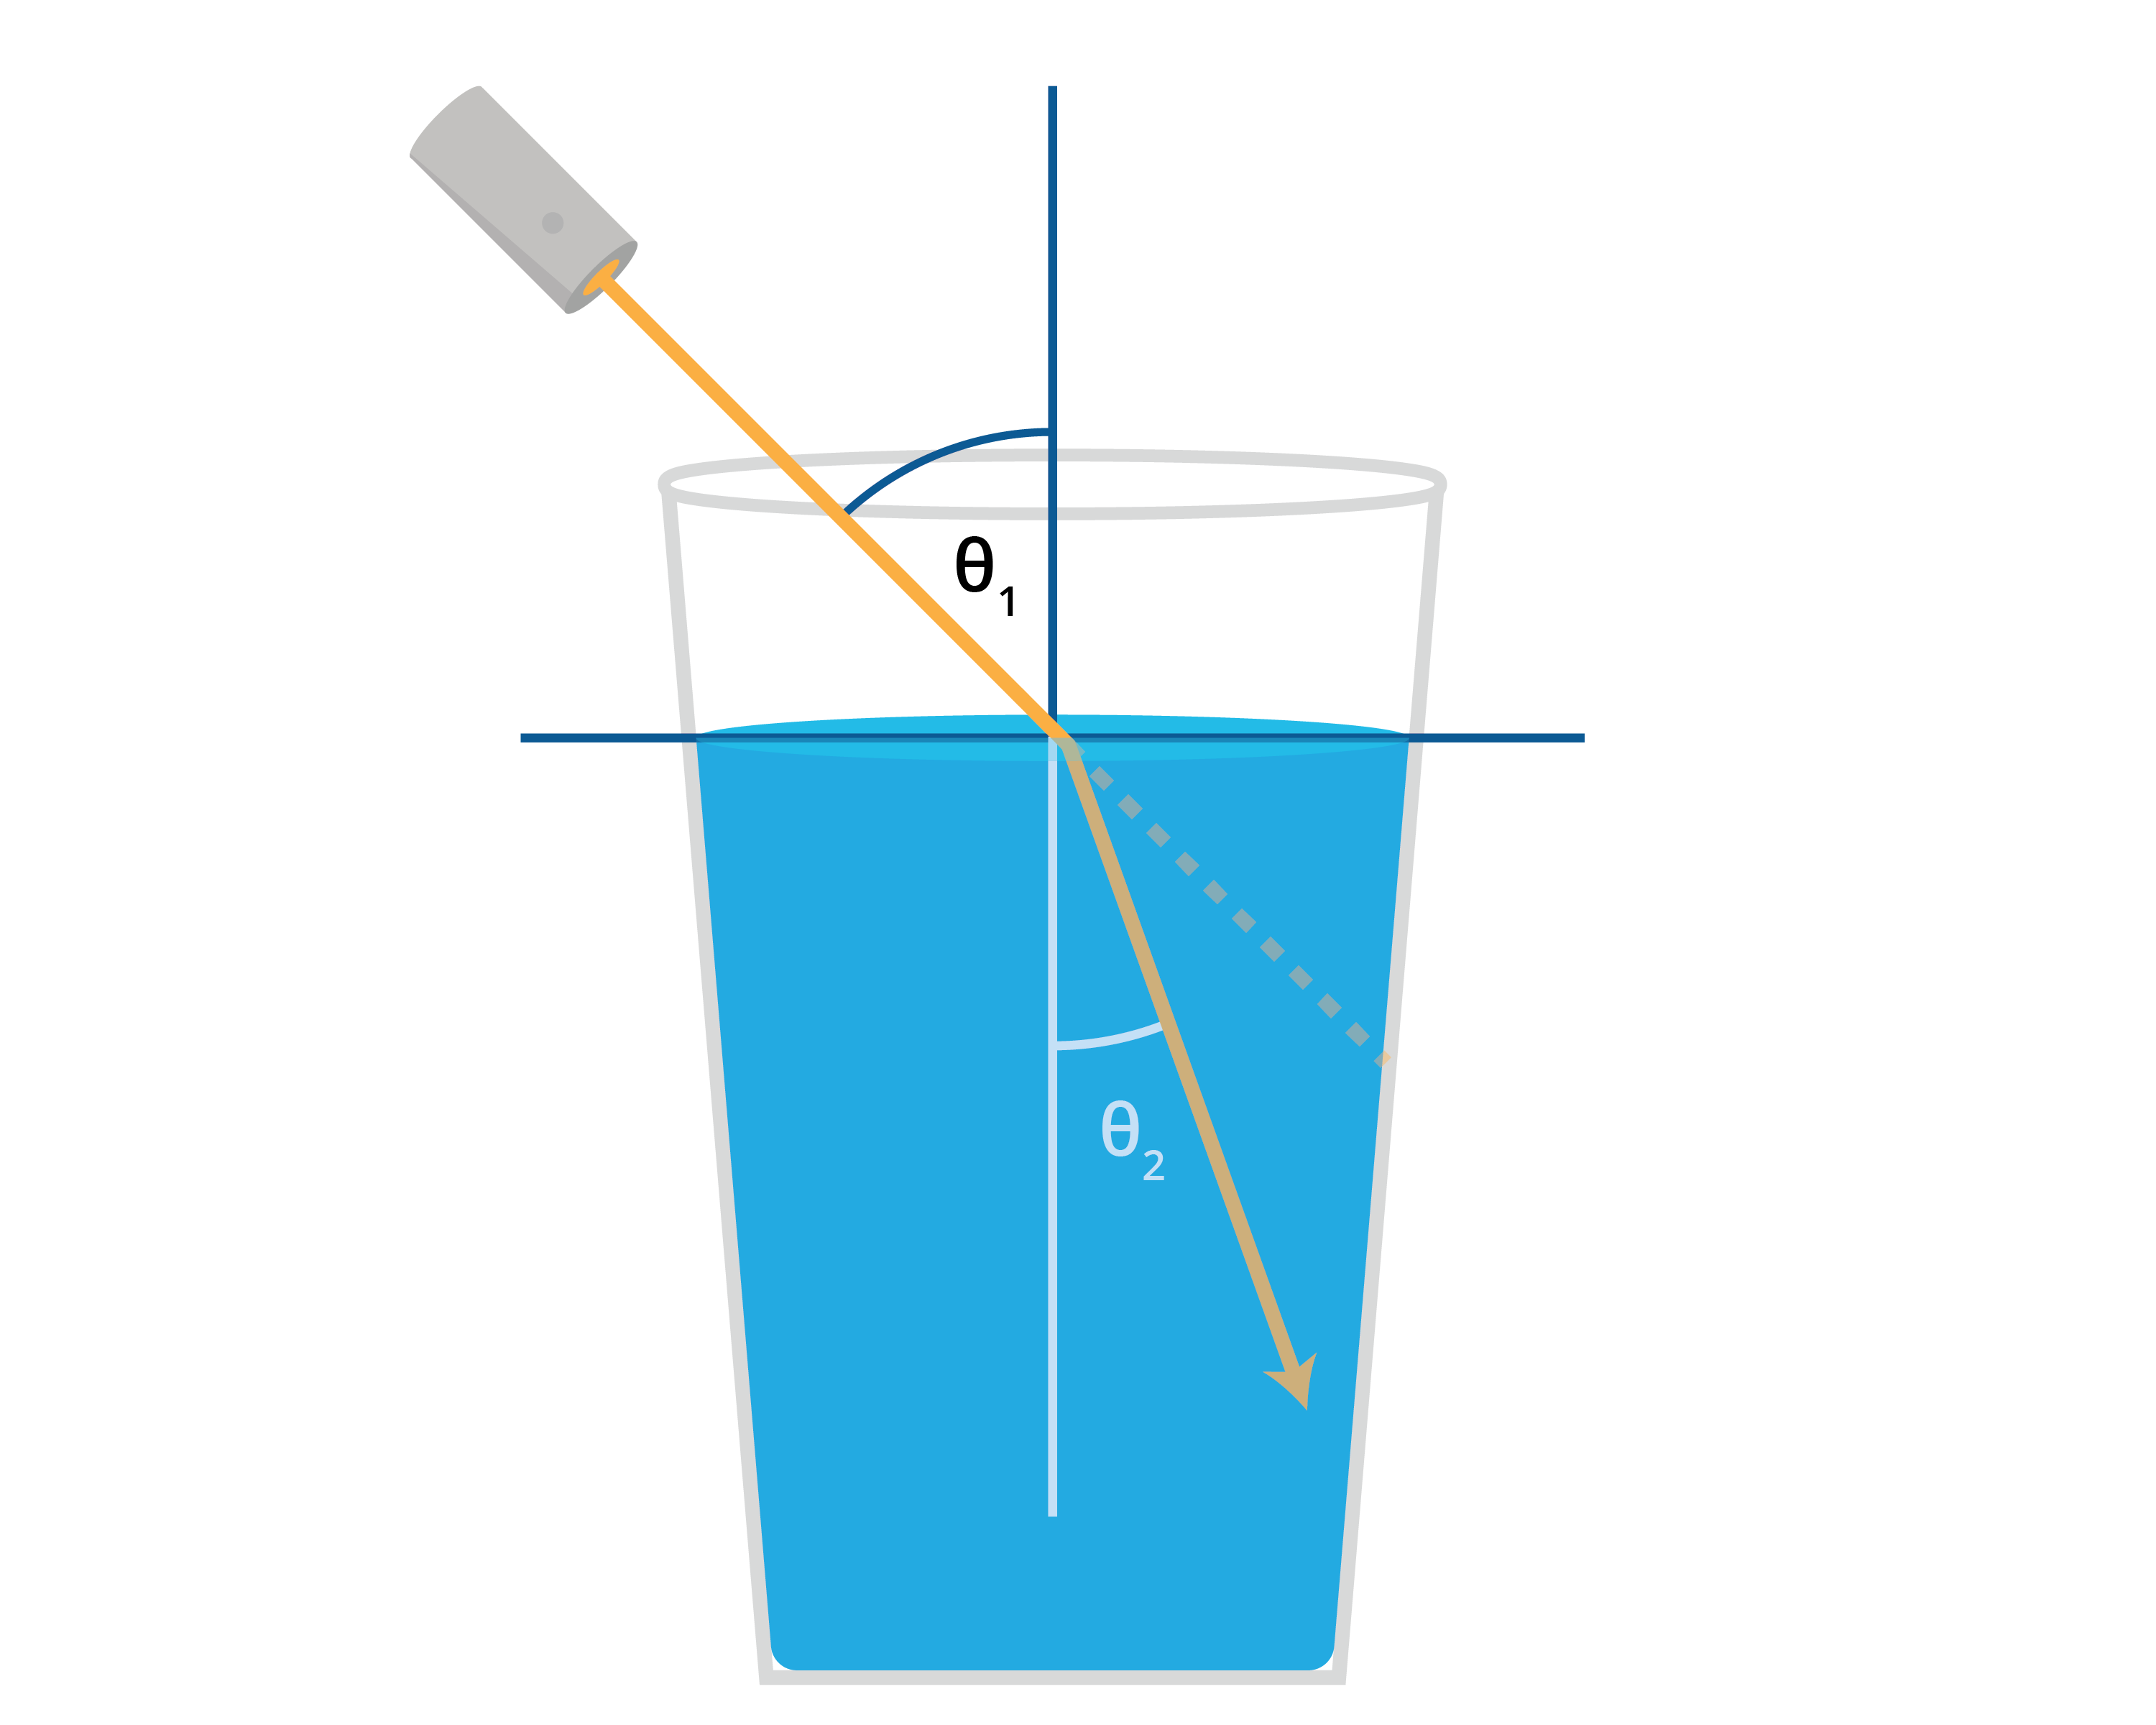
\includegraphics[width=.75\textwidth]{refraction.png}
    \caption{Refraction occurs when light changes the medium it is in.}
    \label{fig:refraction}
\end{figure}

The angle of incidence ($\theta_1$) is the angle between the incident ray and the normal to the interface at the point of incidence. Similarly, the angle of refraction ($\theta_2$) is the angle between the refracted ray and the normal.

When light travels from a medium with a lower refractive index to a medium with a higher refractive index, it bends towards the normal. Conversely, when light travels from a medium with a higher refractive index to one with a lower refractive index, it bends away from the normal.

